\chapter{Processing Sheet Music}

\label{Chapter:Processing-Sheet-Music}
\lhead{\emph{Processing Sheet Music}}

\newcommand{\element}[1]{{\textit #1}}

\section{Introduction}
MusicXML\citep{good2001musicxml} is a music notation interchange format. Nowadays, most commercial music software support this format so we can use it to interchange sheet music between different software. Before MusicXML, the universal music notation interchange format is MIDI. However, a midi file don't contain enough information for rendering sheet music. For example, the direction of note stem is not stored in midi file . Another example is that a note with specific pitch can be represented differently, with the alternating symbols such as sharp, flat and natural, etc.

As the website of MusicXML states, there are more than 170 applications include MusicXML support. Also, more and more scores in MusicXML format are available in digital music databases. All input data comes from the MuseScore \footnote{musescore.com} website. 

\section{Parsing MusicXML}
MusicXML, as its name implies, is an XML based format. We have a wide range of XML libraries available in different programming languages.
Though we can use XML libraries to load the XML file, there are still some work to put on the semantic analyzing of the musical content. 
\subsection{Semantic Parsing}
Semantic parsing is a process that converts data from the storage format to internal format. By internal format, we mean a format that is easy to use in the application. Since this kind of internal format varies from different application, there are few libraries available for this job. Having such a general library for semantic parsing is actually a reinvention of  a general format. However, MusicXML is already a general format and is intuitive enough so having a new one is not necessary. We explored some open source computer music projects which have MusicXML support and found such internal format. The Music21 library \citep{cuthbert2010music21}  can convert between MusicXML and its own format, but it does not expose its MusicXML class as public API. The Lilypond \citep{nienhuys2003lilypond} project has a script, namely ``musicxml2ly.py'', for converting from MusicXML to Lilypond's ``.ly'' format. Relevant classes used by this script are also not part of the public API and nearly undocumented, so it's not easy to reuse in our application. Combining these facts, we decide to write our own semantic parser for converting data from MusicXML to a format that can be used other parts of our application, such as rendering, sound playing and fingering arrangement. 

MusicXML is strictly defined by an XML schema, which is also well documented. We can study the file format directly from the schema. In MusicXML, a musical score is stored as a tree structure\footnote{MusicXML has two types: time-wise or part-wise. We discuss only part-wise here}. It has the following main hierarchy, listed from the root: 
\begin{itemize}
    \item score
    \item part
    \item measure
    \item note/rest/direction
\end{itemize}

Before we introduce these element types, one thing worth to mention is that MusicXML use tenths as unit. A tenth is 1 / 10 of the distance between two staff lines.

In the following, we will introduce these element types briefly. More details about when an element will be used are in the following sections in this chapter.

\subsection{Score}
The score element is the root element. It provides the information about page layout such as page size and page margins. The scaling between tenths and real world length unit is also specified here.

\subsection{Part}
A part element consists of measure elements. There may be several parts in a score, however, our implementation only supports one part. This is because most guitar pieces can be expressed using one part and they are actually expressed using only one part. Using one part does not mean that we can't have polyphony music since MusicXML can put chords in a single part. This will be explained in \ref{section:measure}.

\subsection{Measure}
\label{section:measure}
The measure element is the most complex part of MusicXML. The most essential elements in it are notes, rests and direction. It also contains information about time signature, key signature and tempo.

The timing mechanism inside a measure works by maintaining a time counter with time changing instructions. When a measure is entered, the time counter is set to zero. Then, when each note(or rest) is added, the time counter increase the amount of the note's duration. From this aspect, a note's occurrence can be viewed as a time changing instruction. To support polyphony music, MusicXML has the ``backup'' and ``forward'' instructions. When a backup Instruction is processed, the time counter decrease an amount stated by the instruction. A forward instruction is processed in a similar way, but make the time counter goes forward instead.

\subsection{Note}
A note element tells us the pitch, duration and display style of the note. Unlike the MIDI format, which represents a pitch by an integer proportional to the logarithm of the physical pitch value, pitch in MusicXML is represented by a (step, octave) pair. A step can be one of (C, D, E, F, G, A, B) and octave is an integer.

A note element also tells about accidentals, dots, stems, beams, etc. Further details will be explained in \ref{section:rendering-sheet-music}.

\subsection{Other Symbols}
There are some other types of symbols on a musical score, such as time signature, key signature, text, etc. These symbols are usually straightforward to handle since they do not depend on each other.

\section{Internal Data Representation}
We adopt an object-oriented style in our internal data representation design. As mentioned above, MusicXML has the score-part-measure-note hierarchy. Instead of following the MusicXML hierarchy strictly, we decide to have a sheet-page-measure-note hierarchy. Miscellaneous symbols is attached to measures and notes.
% XXX: class diagram.

One challenge of dealing with MusicXML is that some information is optional, so we need to infer its default value from the context. For example, the distance between a measure and the measure below it may be omitted, then we need to infer this distance value from the previous measures. Sometimes we even have to hard-code default values inside our application. For example, tempo value is optional in MusicXML. However, without this value we cannot convert the music time to actual physic time, which is needed in the following work..

\section{The Parsing Procedure}
In the parsing procedure, a ParseContext is maintained. A ParseContext consist of these values:
\begin{itemize}
    \item sheet: Current sheet.
    \item page: Current page.
    \item measure: Current measure.
    \item beams: A lookup table for beams parsing.
    \item endings: A lookup table for endings parsing, similar to beams.
\end{itemize}

To parse a MusicXML file, we follow the steps below:
\begin{enumerate}
    \item Load the MusicXML schema file.
    \item Load the MusicXML file.
    \item If the file is compressed, decompress it.
    \item Validate the file using the loaded schema.
    \item Initialize the parse context.
    \item Iterate through each measure element in the only part element.
    \item For each measure, if it indicates that a new page should be created, create one.
    \item For each child of the measure node, get the type of this child and use the corresponding handler to handle.
\end{enumerate}

Most of these steps are straightforward: We just read data from the elements and store them to the objects.


\section{Rendering Sheet Music}
\label{section:rendering-sheet-music}

\subsection{Overview}
Sometimes a picture is worth a thousand words. Figure \ref{fig:score-overview} is an overview of the elements on the score. 
\begin{figure}[h]
    \centering
    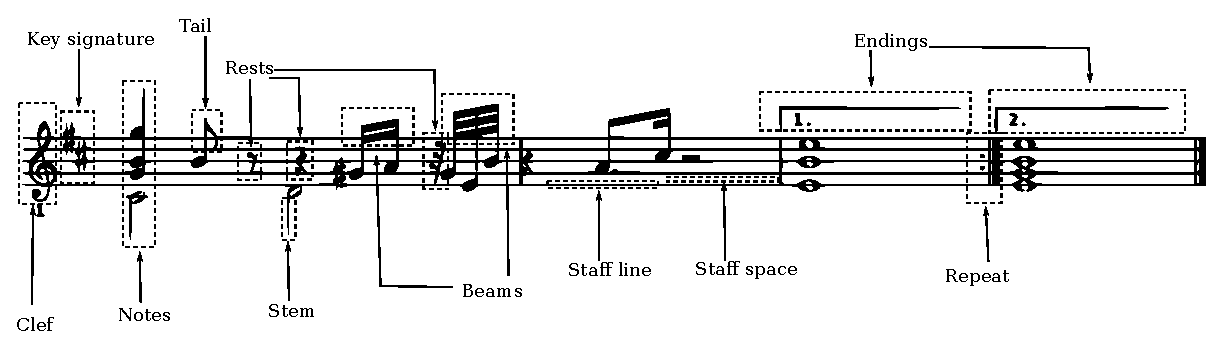
\includegraphics[scale=0.7]{Figures/score-overview.eps}
    \caption{A sample score for illustration purpose}
    \label{fig:score-overview}
    \startdescription
    Elements are highlighted and labeled with names. This sample is rendered by our rendering program and then processed with Inkscape.
\end{figure}

The fundamental part of a score are the staff lines. Each group of staff lines are five parallel long horizontal lines, forming a grid system for other musical elements. At the beginning of a staff, there's usually a clef followed by the key signature. For guitar pieces, usually the G clef is used. 
A staff is split into measures by the vertical bar lines. A measure helps the reader to group notes and to calculate the time. Each measure has its index number, counting from 0 or 1. It counts from 0 when the measure is partial. Although every measure has an index number, not all of them are printed and usually only the leftmost measure's index number is printed. With the aid of index number, readers can describe and locate measures efficiently. 

The vertical bar lines splitting the measures may have different style. They may be thin or thick, single or double. Thin bar line is the one that used most frequently. They are used to split measures.
 Thick bar lines are used at the end of a score. Double bar lines that company with double vertical dots, denote start or end of a repeat.

 Musical notes, along with the stem and beams connecting them, is the most complex part. Details about them will be covered in the following discussion.

\subsection{Primitive Types}
Before we continue on discussing how to render different musical elements, it's worthwhile to classify different primitives.

A typical musical score are printed using only the black color.
So in our model all primitives are rendered using the same color, black.

In our model, all musical elements can be decomposed into these four primitives:
\begin{itemize}
    \item Lines: Both vertical and horizontal.
    \item Beams: Beams is a special kind of line, with their two ends slanted.
    \item Texture: For example, clefs, quarter note heads, full note heads, tails, rests, accidentals.
    \item Text.
\end{itemize}

A line is actually drawn as a long thin rectangle. Formally, a ``line'' here should be called as a segment since it's not infinite. However, we call it a ``line'' for simplicity's sake.
We use 5 variable to describe a line, they are:
    $$(x_1, y_1, x_2, y_2, \mathrm{thick})$$
This is illustrated by Figure \ref{fig:primitive-line}. One remarkable thing is that we found it important to keep the line ends sharp instead of bevel. This is because bevel ends are hard to align with other elements, causing artifacts in the final render result.

\begin{figure}[b]
    \centering
    \begin{minipage}[t]{.5\textwidth}
        \centering
        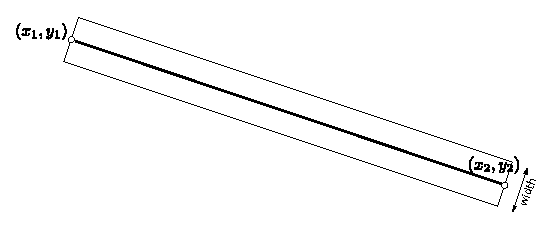
\includegraphics[scale=.8]{Figures/primitive-line.eps}
        \caption{Illustration of line representation.}
        \label{fig:primitive-line}
    \end{minipage}%
    \begin{minipage}[t]{.5\textwidth}
        \centering
        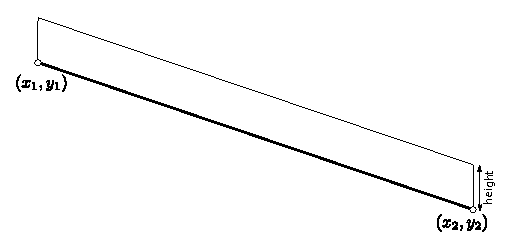
\includegraphics[scale=.8]{Figures/primitive-beam.eps}
        \caption{Illustration of beam representation.}
        \label{fig:primitive-beam}
    \end{minipage}
\end{figure}

\begin{figure}[h]
    \centering
    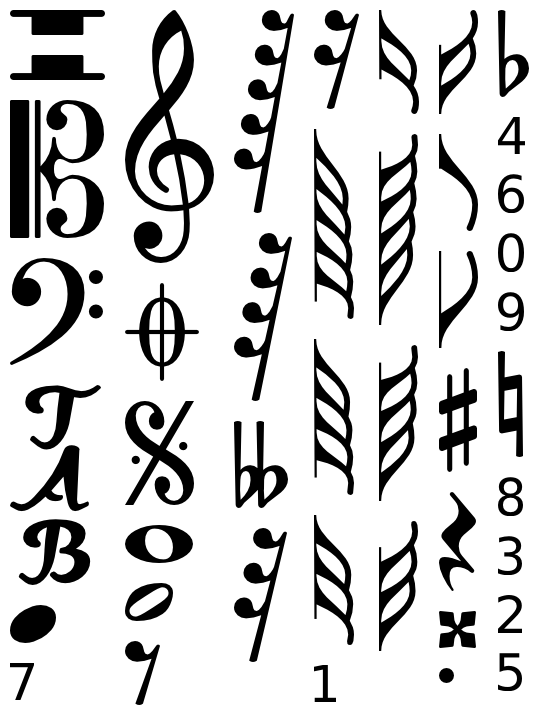
\includegraphics[scale=0.2]{Figures/primitive-texture.png}
    \caption{Packed textures}
    \label{fig:primitive-texture}
    \startdescription
    Each template comes from the Lilypond project. They are rendered into SVG format and then converted to 500dpi PNG image.
\end{figure}

Beams look like lines, except that their ends are slanted. Also, they are attached to the stems most of the time. If we keep using $(x_1, y_1, x_2, y_2, \mathrm{thick})$ to represent a beam, it results that we keep subtracting and adding $\mathrm{thick} / 2$ when calculating
its position. To solve this inconvenience, we use the following representation instead:
\[
    (x_1, y_1, x_2, y_2, \mathrm{height})
\]
The meanings of these variable is illustrated by Figure \ref{fig:primitive-beam}.

To render other elements with irregular shape, we use the template method. First we decompose a complex element symbol into different parts, based on the following rule:
\begin{itemize}
    \item If the symbol has long vertical or horizontal lines, remove it.
    \item For the remaining parts, create a template for each of them.
\end{itemize}
With this method, we get the templates as shown in Figure \ref{fig:primitive-texture}. Since we use OpenGL as the rendering backend, keeping all templates in a single texture image is quite a common way to go. However, packing different templates manually is not easy to maintain, so we make a script using a greedy algorithm to do this. With the help of the script, we can just make each template a single file with its own name, so that we can easily add or remove templates later.

Each template is represented by:
\[
    (x, y, w, h)
\]
Each template has its pivot point $(x, y)$. This is the coordinate on the final packed image. $w$ stands for ``width'', and $h$ for ``height''. 

Texts are rendering in a similar way like textures, so we will not discuss it further here.

\subsection{Note}
Notes are the essential part of the score. The pitch of each note is specified by its vertical position and the duration is specified by both its head shape and its tail.

There exist 3 types of note heads. They're for full notes, half notes, and other notes, respectively. Full notes don't have stems connected, and the head is a bit larger than other notes. Half notes look like quarter notes, except that their heads are hollow. Notes with duration less than quarter has the same note heads since their duration is then not distinguished by their heads, but their tails instead. As a result, we need to prepare only 3 templates for note head rendering.
 
A note is usually connected by a stem, which heads up or down and has various length. The direction of a stem is told by MusicXML. Different directions of a stem is used to distinguish between different voice parts. While the head position of a stem is determined by the note head and the stem direction, the tail of it is determined by the beam attached to it, if it has any. A stem without beams can be any visually proper length. We use 35 tenths as this default value in our application. 

A single stem may be connected to multiple notes. This is often seen in chords. Examples can be found in Figure \ref{fig:score-overview}.

\subsection{Beams}
Beams are for telling the duration of notes and for grouping notes. Grouped notes can express the indent of the composer. A note \footnote{Here we are discussing notes with quarter note head since full notes and half notes don't have beams. } without any beams but only a stem have the duration of 1/4. When one more beam is attached, the duration is divided by 2. It's not hard to get the conclusion that a note with $n$ beams have duration of $1 / 2^{n+2}$.

Usually, in musical score, beams has different slopes, which is determined by vertical positions of notes that they connect. However, the rules to determine the slope is seldom mentioned. Some software just let the slope be 0. This is, they render all beams horizontally, which makes the score look weird and don't comply with the musical convention. 

Here comes three observations that build up the fundamental rules of our method:
\begin{enumerate}
    \item 
        Beams that connected to common stems and have common horizontal span should have the same slope.
    \item
        A proper slope for a beam should make the length of stems connecting to the beam as uniform as possible. 
    \item 
        There should be only several slope value used in rendering since using too many slope value will mess up the score, which is not ideal.
\end{enumerate}


A beam can be partial or complete. Partial beams can then be divided into forward and backward beams. Partial beams cannot occur by itself since a beam occur by itself is actually a tail, which is rendered differently. With this observation, we can assume that partial beams can always be drawn after complete beams.

A beam may be connected to up stems or down stems, but rarely both. We can assume that all stems that a beam connected to have the same direction. Then we have two types of beam, one with up stems and the other with down stems. Since the calculation between these two types are similar, from this point on we discuss about only the type that has up stems.

In our beam slope calculating algorithm, we have two important concepts:
\begin{itemize}
    \item Length:
the length of a beam is defined as the number of different stems that connected to it. 
    \item Anchor:
        An anchor is a stem that its tail position is determined.
\end{itemize}

Note that if a beam's slope is calculated, the slope of beams below or above it should be the same value. So if we sort the beams by their length, from long to short, and then assign their slope, then we only need to calculate the topmost one in each group of beams. With the aid of anchors, sometimes we can determine the slope of a beam directly. Details is covered in the algorithm listing. \ref{algo:layout-beams}.

\begin{algorithm}
    \caption{Layout Beams and Stems} \label{algo:layout-beams}
    \begin{algorithmic}[1]
        \State Sort beams by length, from long to short.
        \For{ beam $\in$ beams }
            \State anchors $\gets$ Next available position from all up stems connected to beam.
            \If{length of anchors $\ge$ 2}
                \State anchorL $\gets$ leftmost anchor from anchors
                \State anchorR $\gets$ rightmost anchor from anchors
                \State Set the two ends of the beam to anchorL and anchorR, respectively.
            \Else
                \State tails $\gets$ tail positions of stems connecting to beam
                \State $e_m \gets \inf $ \Comment{Current minimum error value}
                \State $ A \gets \left[\begin{array}{cccc}
                        x_1 & x_2 & \cdots & x_n \\
                        1 & 1 & \cdots & 1 \\
                    \end{array}\right]^T$
                \State $ B \gets \left[\begin{array}{cccc} 
                        y_1 & y_2 & \cdots & y_n 
                    \end{array}\right]^T$

                \For{ $k \in \left\{-0.2, -0.1, -0.05, 0.05, 0.1, 0.2\right\} $}
                    \State bLimits $\gets B - k A[:, 0]$
                    \State $ b \gets max(\mathrm{bLimits}) $
                    \State $ \vec{x} \gets (k, b) $
                    \State $ e \gets \left|Ax - B \right|^2 $
                    \If{$e < e_m$}
                        \State $e_m \gets e$
                        \State $\vec{x}_m \gets \vec{x} $
                    \EndIf
                \EndFor
                \State $(k, b) \gets x_m$

                \State $\vec{p_1} \gets k x_1 + b $
                \State $\vec{p_2} \gets k x_n + b $
                \State Set the two ends of the beam to $\vec{p_1}$ and $\vec{p_2}$, respectively.
            \EndIf
        \EndFor
        
    \end{algorithmic}
\end{algorithm}

After this algorithm is performed, we can determine both beam positions and stem positions relative to the measure.

\subsection{Accidentals and dots}
Accidental symbols may occur in two places. The first place is the key signature and the other is the area to the left of note heads. Dots that extending a note's duration may only occur to the right of the note. For accidentals and dots around the note head, it's quite straightforward to render. Once the note's position is determined, we just put them around. 

One remarkable optimization for accidental positioning is that we found a way to avoid the overlap of close accidentals. One situation is illustrated by Figure \ref{fig:avoid-accidental-overlap}. To do this, we first sort all accidentals in a measure, from bottom to top, then left to right. Then we start to put accidentals onto the measure by the sorted order. When an accidental overlap with other ones, move it to left by half of it's width, until there's no overlap. However, to avoid an accidental be moved too far from its original position, we constraint the count of moves to 5 for each accidental. Here, the collision detect can use the brute force way, with $O(n^2)$ time complexity, where $n$ is the number of accidentals in the measure. Since there's always only a few accidentals in each measure, this method will work well.

\begin{figure}[h]
    \centering
    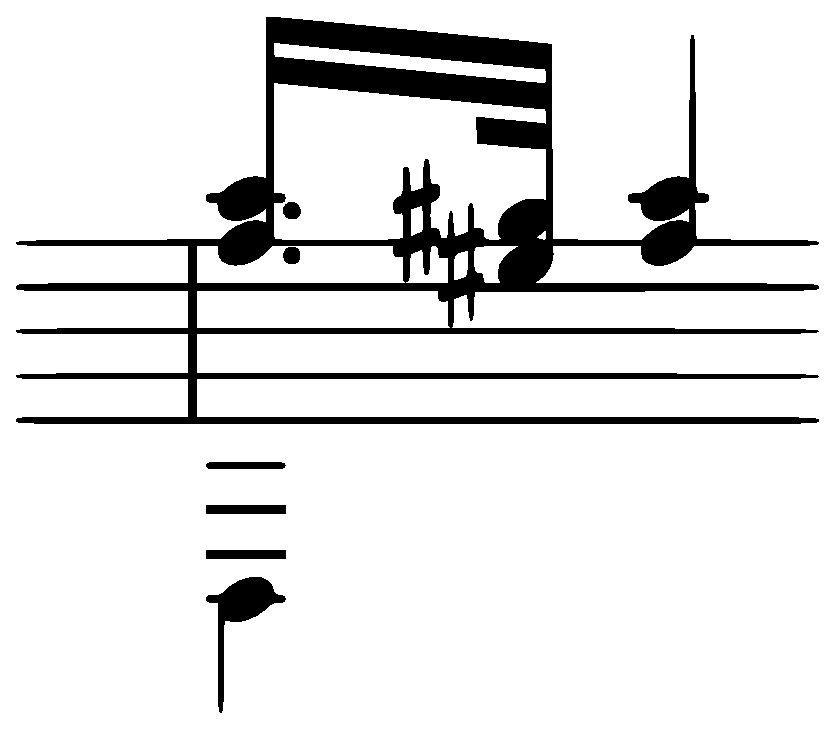
\includegraphics[width=0.4\textwidth]{Figures/accidental-overlap.eps}
    \caption{Avoiding accidental overlap}
    \label{fig:avoid-accidental-overlap}
\end{figure}
For the accidental symbols used in key signature, there is a set of conventional rules. The writing of key signature is relevant to the clef. Here we only discuss the G clef situation, for the sake of simplicity. In most guitar pieces we only use the G clef.

\subsection{Key Signature}
In MusicXML, the musical key is described by fifths and octave. When the center of G clef is aligned with the second staff line(counting from bottom to top), and if the octave is 3, we know that the second line correspond to the pitch G3. The variable fifths tells about how many fifths we have and what's the accidental type. If fifths is positive, then the type is sharp. If  fifths is negative, then we have flat fifths. For example, if fifths is 1, we know that there is only one sharp, which means the key is G major. If fifths is 2, we know that there are two sharps, and the key is D major. If fifths is -2, we know that there are two flats, and the key is Bb major. The fifths variable can range from $-7$ to $7$. Table \ref{table:fifths-sharp} and \ref{table:fifths-flat}  show the correspondence between fifths and key signatures.

\begin{table}[h]
    \centering
    \begin{tabular}{r|r|l}
        Fifths & Key & Sharps \\
        \hline
        0 & C major &\\
        1 & G major & F\#\\
        2 & D major & F\#, C\#\\
        3 & A major & F\#, C\#, G\#\\
        4 & E major & F\#, C\#, G\#, D\#\\
        5 & B major & F\#, C\#, G\#, D\#, A\#\\
        6 & F\# major & F\#, C\#, G\#, D\#, A\#, E\#\\
        7 & C\# major & F\#, C\#, G\#, D\#, A\#, E\#, B\# \\
    \end{tabular}
    \caption{Table of sharp fifths}
    \label{table:fifths-sharp}
\end{table}

\begin{table}[h]
    \centering
    \begin{tabular}{r|r|l}
        Fifths & Key & Flats\\
        \hline

        -1 & F major & Bb\\
        -2 & Bb major &Bb, Eb\\
        -3 & Eb major &Bb, Eb, Ab\\
        -4 & Ab major &Bb, Eb, Ab, Db\\
        -5 & Db major &Bb, Eb, Ab, Db, Gb\\
        -6 & Gb major &Bb, Eb, Ab, Db, Gb, Cb\\
        -7 & Cb major &Bb, Eb, Ab, Db, Gb, Cb, Fb \\
    \end{tabular}
    \caption{Table of flat fifths.}
    \label{table:fifths-flat}
\end{table}

With these two table, we can know which sharp or flat should be added and their order. However these information is not enough for us to decide their position. For example, in G major we have one sharp fifths. Looking up from Table \ref{table:fifths-sharp}, we know that it's F. However, both the space above the first staff line and the fifth staff line are in pitch ``F'', so it's possible to put the sharp symbol on both places, or even more places. Actually, sound F in G clef key signature is by convention drawn on the fifth line. So we need another table, as shown in Figure \ref{fig:key-signatures}. With this table, we now know the vertical position for each symbol to put.

\begin{figure}[t]
    \centering
    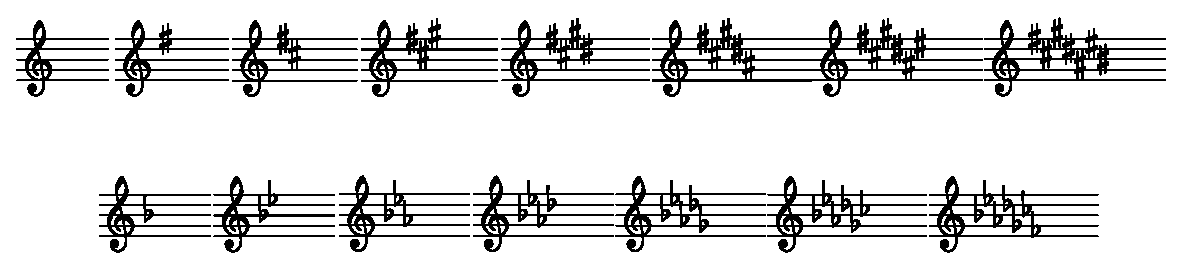
\includegraphics[scale=0.72]{Figures/key-signatures.eps}
    \caption{Different key signatures.}
    \label{fig:key-signatures}
    \startdescription

    First line correspond to fifths with value range from 0 to 7. 
    Second line correspond to fifths with value range from -1 to -7.
\end{figure}

\subsection{Other Symbols}
There are other symbols in a score, such as bar lines, endings, title, etc. We will not discuss them here since they are quite straightforward to handle.

\subsection{Rendering Order}
Here is a short summary of the rendering order of elements discussed above.
\begin{itemize}
    \item Staff lines
    \item Clef
    \item Key signature
    \item Notes
    \item Beams and stems
    \item accidentals
    \item Bar lines
    \item Endings
\end{itemize}


\section{Results}
We will discuss the result through examples. Each of these examples are some consecutive measures from various scores, rendered by our rendering engine. Each example will be used to illustrate a feature of our rendering engine. All origin MusicXML scores are downloaded from the MuseScore website.

\newcommand{\renderscale}{0.3}

\begin{figure}[h]
    \centering
    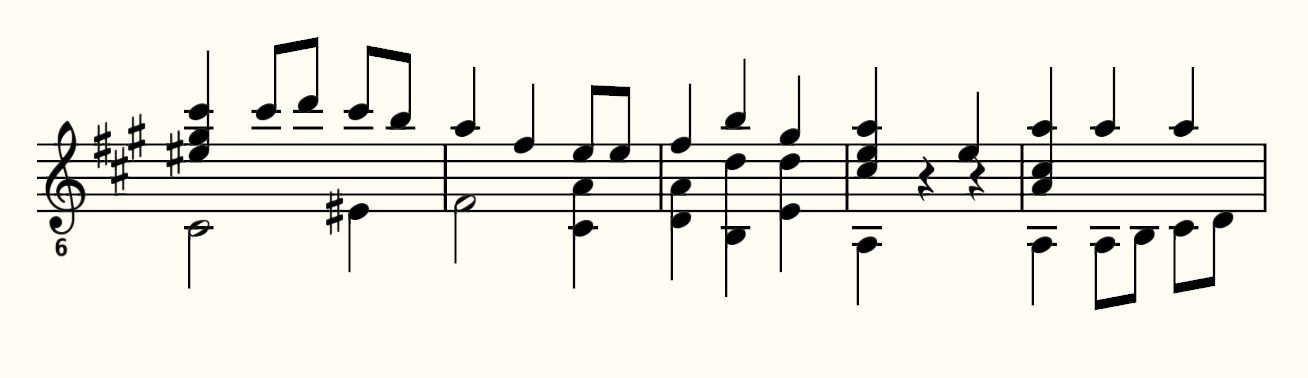
\includegraphics[scale=\renderscale]{Figures/render-we-wish-you-a-merry-christmas.png}
    \caption{An overview of render result.}
    \label{fig:render-overview}
\end{figure}

\begin{figure}[h]
    \centering
    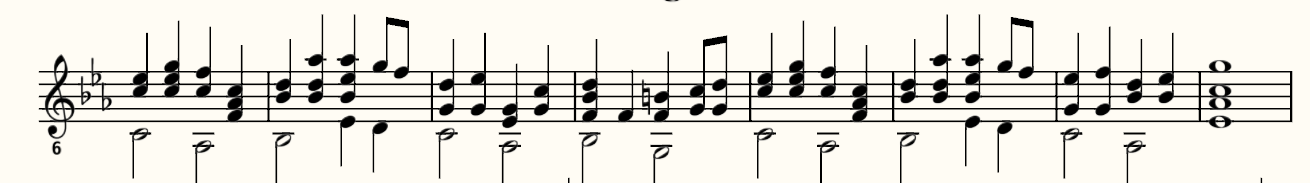
\includegraphics[scale=\renderscale]{Figures/render-People-Imprisoned-by-Destiny.png}
    \caption{Example with dense measures.}
    \label{fig:render-dense}
    \startdescription
     The example illustrates the result of rendering chords. In a chord, multiple note heads are attached to the same stem. The length of a stem need to be extended properly to support more notes.
\end{figure}


% \begin{figure}[h]
%     \centering
%     \includegraphics[scale=\renderscale]{Figures/render-<++>.png}
%     \caption{<++>}
%     \label{fig:render-<++>}
%     \startdescription
%     <++>
% \end{figure}<++>

\begin{figure}[h]
    \centering
    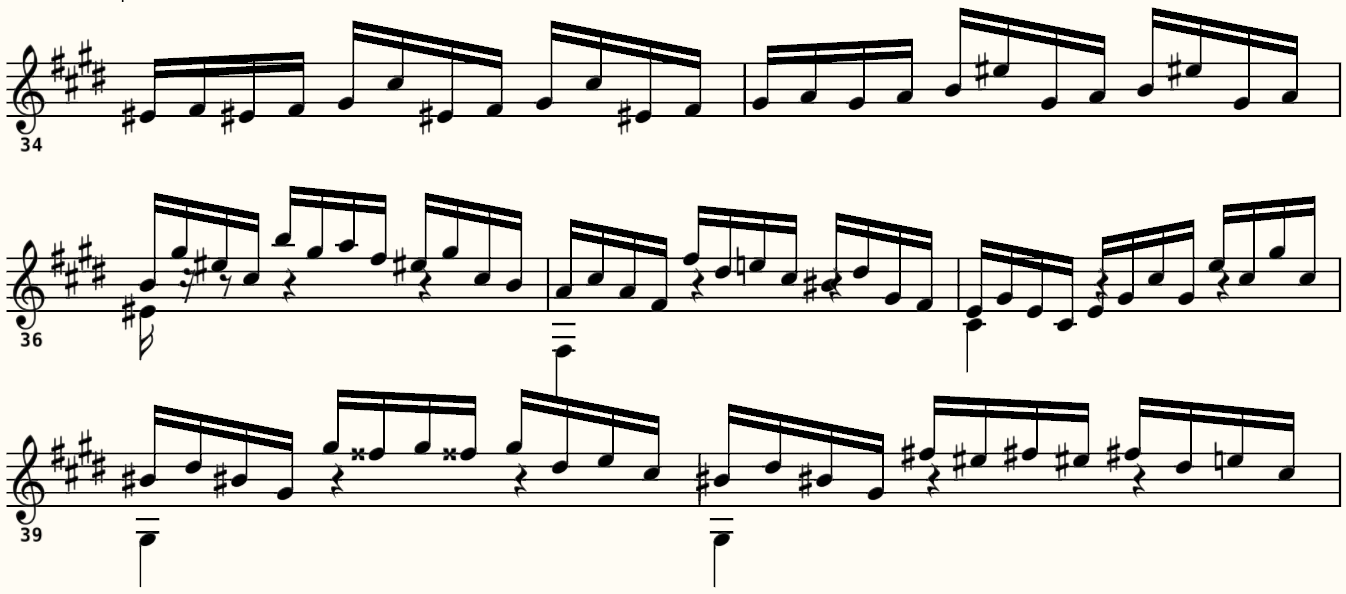
\includegraphics[scale=\renderscale]{Figures/render-Allegro-by-Bernardo-Palma-V.png}
    \caption{Render result for multiple beams.}
    \label{fig:render-multiple-beam}
    \startdescription
    In this example we can see that the slope of a beam is affected by the notes.
\end{figure}


\begin{figure}[h]
    \centering
    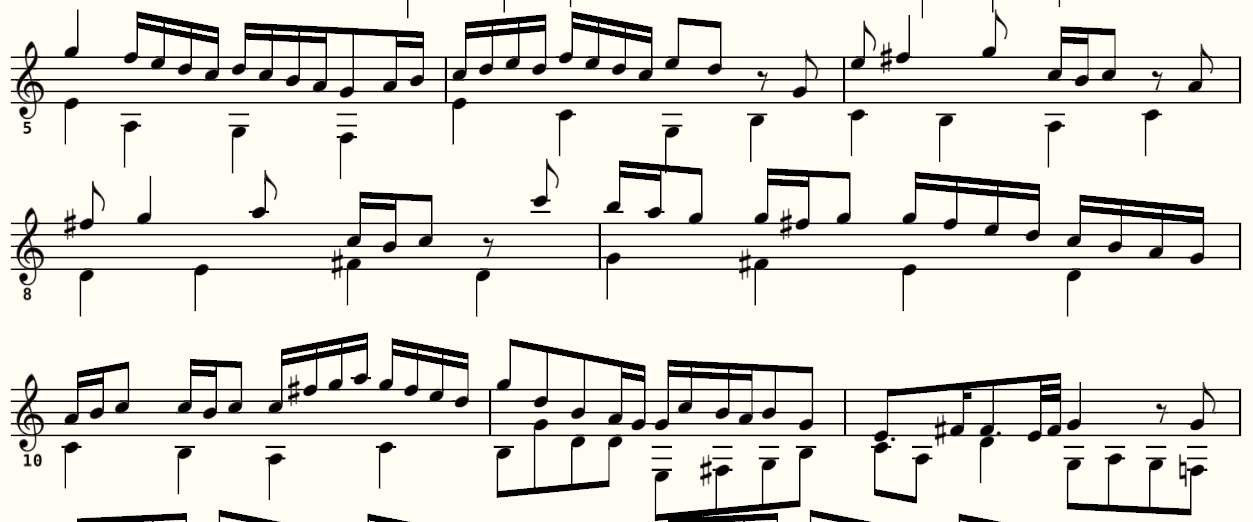
\includegraphics[scale=\renderscale]{Figures/render-BWV-645-C.png}
    \caption{Measures that contains beams with different length in the same group.}
    \label{fig:render-beam-vary-length}
    \startdescription
    In the first measure(with measure number 5), there is even more than one short beams under the long beam in the same group. We can see here our algorithm handled these situation properly.
\end{figure}

\begin{figure}[h]
    \centering
    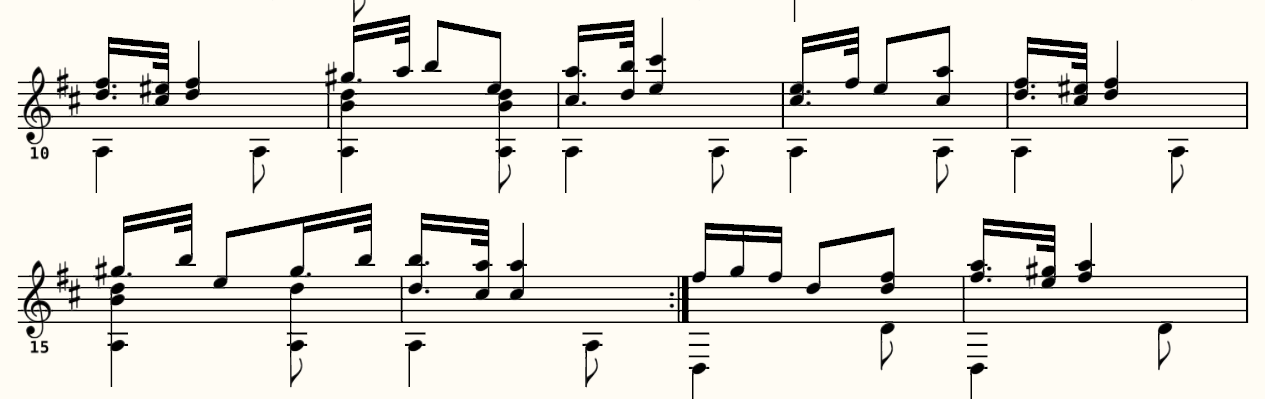
\includegraphics[scale=\renderscale]{../Figures/render-Fernando-Sor-Op-32-Mazurka.png}
    \caption{Example with complex beams.}
    \label{fig:render-complex-beams}
    \startdescription
    In this example we can find that partial beams are rendered properly in groups with multiple levels of beam. In the first measure of second row, the second group of beams, which is more complex than others, is also rendered properly.
\end{figure}

\begin{figure}[h]
    \centering
    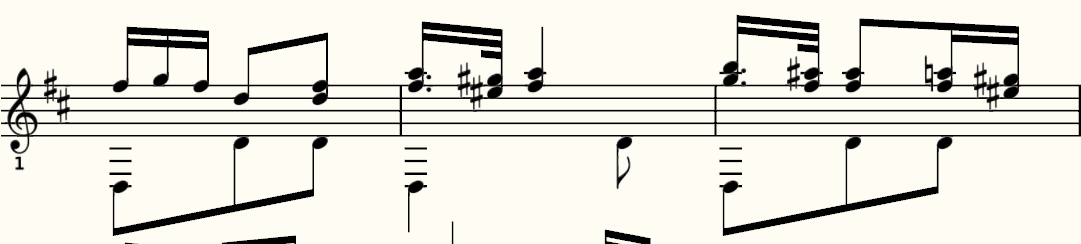
\includegraphics[scale=\renderscale]{Figures/render-Fernando-Sor-Op-32-Mazurka-1.png}
    \caption{Example to illustrate the accidental positioning optimization.}
    \label{fig:render-accidental}
    \startdescription
    In the second and third measure we can see that the sharp symbol are placed properly without overlapping. Even if they are very close to each other.
\end{figure}


\begin{figure}[h]
    \centering
    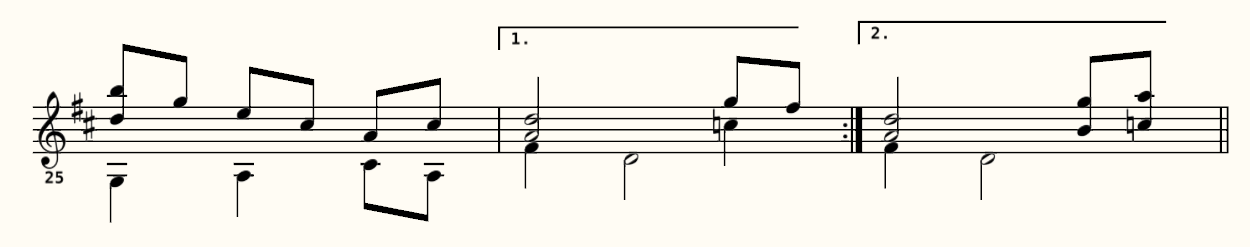
\includegraphics[scale=\renderscale]{Figures/render-Guitar-Solo-No-98-in-D-Major.png}
    \caption{Example with endings.}
    \label{fig:render-endings}
\end{figure}
